%%*************************************************************************
%% Legal Notice:
%% This code is offered as-is without any warranty either expressed or
%% implied; without even the implied warranty of MERCHANTABILITY or
%% FITNESS FOR A PARTICULAR PURPOSE! 
%% User assumes all risk.
%% In no event shall IEEE or any contributor to this code be liable for
%% any damages or losses, including, but not limited to, incidental,
%% consequential, or any other damages, resulting from the use or misuse
%% of any information contained here.
%%
%% All comments are the opinions of their respective authors and are not
%% necessarily endorsed by the IEEE.
%%
%% This work is distributed under the LaTeX Project Public License (LPPL)
%% ( http://www.latex-project.org/ ) version 1.3, and may be freely used,
%% distributed and modified. A copy of the LPPL, version 1.3, is included
%% in the base LaTeX documentation of all distributions of LaTeX released
%% 2003/12/01 or later.
%% Retain all contribution notices and credits.
%% ** Modified files should be clearly indicated as such, including  **
%% ** renaming them and changing author support contact information. **
%%
%% File list of work: IEEEtran.cls, IEEEtran_HOWTO.pdf, bare_adv.tex,
%%                    bare_conf.tex, bare_jrnl.tex, bare_jrnl_compsoc.tex
%%*************************************************************************

\documentclass{llncs}
%\documentclass[10pt, conference, compsocconf]{IEEEtran}

\usepackage{ucs}
\usepackage[utf8x]{inputenc}
\usepackage[english]{babel}
\usepackage{hyperref}     % use \url{http://$URL} or \href{http://$URL}{Name}
\usepackage{underscore}   % underscores need not be escaped
\usepackage{subfigure}
\usepackage{verbatim}
\usepackage{moreverb}
\usepackage{float}
\usepackage{booktabs}     % professional tables
\usepackage{listings}
\usepackage{color}
\usepackage{amsmath}
\usepackage{indentfirst}
\definecolor{darkgreen}{rgb}{0,0.4,0}
\lstset{language=C,captionpos=b,tabsize=3,frame=lines,keywordstyle=\color{blue},commentstyle=\color{darkgreen},stringstyle=\color{red},numbers=left,numberstyle=\tiny,numbersep=5pt,breaklines=true,showstringspaces=false,basicstyle=\footnotesize,emph={label}}

% Support for including graphics
\usepackage{graphicx}
\DeclareGraphicsExtensions{.pdf,.png,.jpg}

\begin{document}

\title{Detection of Encrypted Android Malware Using Dalvik Hooks}

%\author{\IEEEauthorblockN{Ionuț-Mihăiță Pleșea, Silviu-Mihai Popescu}
%\IEEEauthorblockA{Computer Science and Engineering Department\\
%University POLITEHNICA of Bucharest\\
%Bucharest, Romania\\
%\emph{\{ionut.plesea, silviu.popescu\}@cti.pub.ro}}
%}

\author{Ionuț-Mihăiță Pleșea, Silviu-Mihai Popescu}
\institute{Computer Science and Engineering Department\\
University POLITEHNICA of Bucharest\\
Bucharest, Romania\\
\email{\{ionut.plesea, silviu.popescu\}@cti.pub.ro}}

% make the title area
\maketitle


\begin{abstract}
  % vim: set tw=78 sts=2 sw=2 ts=8 aw et ai:
There are several layers of analysis and isolation in the Android application
environment, all develope with the explicit purpose of ensuring that the
features of smartphones do not expose personal user information to malicious
third parties. While the current set of barriers covers many attack vectors,
the solutions are limited if the malware is delivered to the victim device as
a seemingly inoffensive file only to be transformed using cryptographic
primitives into a malicious application package. Since the
transformation is done on the victim device, most safeguards are bypassed. We
propose a system that detects tentative attacks which use the above mentioned
approach by instrumenting the cryptographic primitives in order to
detect if both input and output are valid files.

\end{abstract}

%\begin{IEEEkeywords}
%Android, Dalvik, cryptography, malware, method hooking, AngeCryption,
%instrumentation
%\end{IEEEkeywords}
\keywords{Android, Dalvik, cryptography, malware, method hooking, AngeCryption,
instrumentation}

% For peerreview papers, this IEEEtran command inserts a page break and
% creates the second title. It will be ignored for other modes.
%\IEEEpeerreviewmaketitle

\section{Introduction}
\label{sec:intro}
% vim: set tw=78 sts=2 sw=2 ts=8 aw et ai:

Having been on the market for 6 years, the Android operating system and the
environment around it have evolved continuously in reply to user demand. With
this growth in popularity the need for providing adequate security for
personal data has been increasingly pronounced.

While safety mechanisms have always been present in Android, it was only
recently\cite{android-layers} that the Android Security Team highlighted the
protection features available on more than half of the smartphones sold
globally. A summary can be seen in Figure \ref{fig:layers}. With so many
checks and analysis being done both on Google servers and on the device
itself, successfully compromising a smartphone is increasingly difficult for
an attacker and consequently innovative manners of bypassing these filters
have been developed.

\begin{figure}[hb]
  \centering
  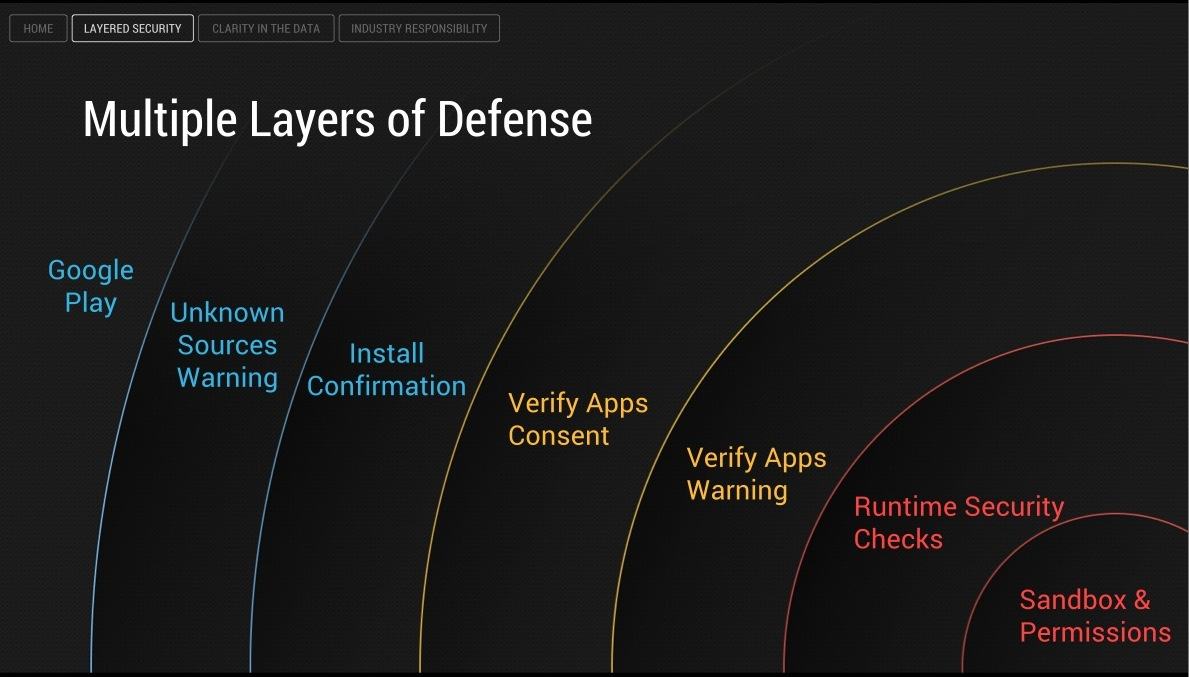
\includegraphics[width=0.5\textwidth]{img/android-layers}
  \caption{Android Security Layers - Image courtesy of Andrian Ludwig}
  \label{fig:layers}
\end{figure}

One approach employed by malicious agents is to use picture files bundled with
the Android application. Normally pictures are bundled with applications for
cosmetic purposes and therefore ignored and considered harmless. However,
there is nothing preventing a determined attacker to use such a file as a
wrapper for hiding a harmful payload. Basically, the original application is a
trojan, indistinguishable from an ordinary application.

The first incident of this type has been reported in September
2011\cite{droid-coupon}. An application called DroidCoupon pretended to offer
various coupons in order to lure users to download it. However, it used an
image file to hide a local privilege exploit. For all intents and purposes the
special file behaved like an image file, but the DroidCoupon application,
reading from a custom offset, extracted the local exploit and used it to gain
root access on the smartphone. From that point, the attacker could violate
security protections and leak private user data.

As time progressed, so has the complexity of the techniques used by attackers.
In 2013, the Gamex malware also used an image file to hide the malicious
payload\cite{hiding-apk}. However, its approach was a little more elegant. A
file with the PNG extension was, in fact, a ZIP archive and by default would
extract harmless files. Nevertheless, if the ZIP archive was XOR-ed with a
certain key it produced another valid ZIP, which contained the malicious
payload. This was a significand step up from previous incidents, as
recognizing such behavior was not a trivial task.

Last but not least, in 2014, researchers went a step further\cite{hiding-apk}.
Although the behavior of Gamex was atypical, the fact that it used XOR
encryption meant that subsequent tentatives of the same manner could be
thwarted. Therefore, they employed the cryptographic ciphers exposed by the
Android framework in a rather unorthodox manner. In addition, they relied on
the fact that parsers for specific file formats are error-prone. As a result,
they managed to encrypt a PNG file using AES in CBC mode and obtain a valid
APK file, an Android application that could be installed on the victim
software. Using a standardized encryption algorithm to hide the malicious
payload renders any analysis useless as it is computationally infeasible to
crack AES.

Having outlined previous work with regards to the problem we attempt to solve,
we will now take into account prior research that may aid in the development
of an effective countermeasure. Since the current trend seems to be using more
secure cryptographic ciphers, namely the ones provided by the Android
framework itself, we consider instrumenting the framework itself a valid
approach. More to the point, we wrap methods from Android's cryptographic API
and look for valid file headers in both the input and the output. Normally,
depending whether we are encrypting of decrypting, either the input or the
output should have a valid file signature, while the other should seem random.
If both are not random, then there is a high probability that we are
witnessing a tentative attack.

There are a few instrumentation frameworks available for the Android platform.
Most are geared towards modifyig the user interface and adding features. They
provide complex functionality. Therefore, they are not trivial to setup and,
considering out target are cryptographic operations, may add non-negligible
overhead.

Thankfully, security researchers have developed simplified
alternatives. While lacking in features when compared with more
mature instrumentation frameworks, DDI\cite{ddi} is lightweight and will not
induce a high computational overhead. It works by injecting a library in the
Dalvik runtime that replaces the original entry points to the methods of
interest. The Dalvik virtual machine is the part of the Android operating
system that runs the individual applications. Therefore, a wrapper function
here can be applied to the method of our choice in the context of the
application we wish to monitor.


\section{Instrumenting Cryptographic Primitives}
\label{sec:design}
% vim: set tw=78 sts=2 sw=2 ts=8 aw et ai:

TODO


\section{Ciphermon - Monitoring Cipher Operations}
\label{sec:implementation}
% vim: set tw=78 sts=2 sw=2 ts=8 aw et ai:

Since our research covers the Android operating systems, it is natural that
the proposed solution comes as an Android application. To this end, we have
made use of and repackaged Collin Mulliner's Dynamic Dalvik Instrumentation
framework. Full credit is given for his excellent implementation of Dalvik
hooking.

We have looked at the demonstrative application that researchers have
previously\cite{hiding-apk} developed in order to highlight encrypted malware.
While our approach is extensible, we have targeted this specific sample.

\subsection{Tools and Constraints}

The demonstrative application that highlights encrypted malware can be found 
on Github under the name
 \emph{angecrypt}\footnote{\url{https://github.com/cryptax/angeapk}}. 

We wrapped our solution around it so when we designed our hook we specifically 
targeted a function called \emph{doFinal()} \footnote{\url{ 
http://developer.android.com/reference/javax/crypto/Cipher.html\#doFinal()}}
by taking its input and output and comparing them to signatures of known 
file formats (in this particular demonstrative application, the input was a PNG
file and the output a valid APK file). 

We used the Android SDK\footnote{\url{https://developer.android.com/sdk/index.html\#Other}}
to build the Bootup Receiver, the New Application Receiver 
and the Main Application modules, and relied on the Android NDK\footnote{\url{https://developer.android.com/tools/sdk/ndk/index.html\#Downloads}}
when tackling the Hook Injector and the Hook modules.

One of the biggest constrain that we had was the fact that we used an 
emulator instead of a rooted Android phone due to financial limitations 
(warranty voiding due to rooting). Because of this we were unable to fully
 automate the Hook Injector and the hijacking of the above specified 
method had to be done manually.



\section{Results}
\label{sec:results}
% vim: set tw=78 sts=2 sw=2 ts=8 aw et ai:
The main goal, i.e. detecting malicious action being carried out by 
a suspiciuos application (namely angecrypt), of our PoC (Proof-of-Concept)
environment was achieved. We will further expand the process through
 which our result can be reproduced.

\subsection{Setup Tools and Projects}
In order to reproduce our result, a rooted phone is needed or at least an 
emulator that has superuser access. In our experiments, we resorted to 
using an emulator with Android 4.4.2 and API level 19 that was emulating 
an ARMv7 architecture. It is considered implicit the availability of an 
Android SDK as well as an Android NDK.

One would also need the sources of \emph{ADBI}\footnote{\url{https://github.com/crmulliner/adbi}}
and \emph{DDI}\footnote{\url{https://github.com/crmulliner/ddi}} 
projects developed by \cite{ddi}. In order to use our hook instead of the 
examples provided in DDI, our project\footnote{\url{https://github.com/silviupopescu/ciphermon/blob/master/jni/mon.c}} sources have to be dumped in the ddi/examples folder.

Last but not least the suspicious application is required. That can be 
found on Github as well under the name emph{angeapk}
\footnote{\url{https://github.com/cryptax/angeapk/tree/master/wrapping-apk/src/com/fortiguard/poc/angecrypt}}

\subsection{PoC Reproduction}

The suspiciuos APK can be found in the Github repository mentioned above. 
The \emph{adb} tool can be used to install the app on the phone/emulator.
Assuming your are in the angeapk folder:
\begin{verbatim}
adb install PocActivity-debug.apk
\end{verbatim}
will install the APK.

We will now compile binaries that support the hooking platform. We 
need to be in the ADBI folder.
\begin{verbatim}
cd adbi/hijack/jni
ndk-build
adb push ../libs/armeabi/hijack /data/local/tmp/
cd ../..
cd instruments/base/jni
ndk-build
cd ../../../..
\end{verbatim}
Next, we will compile the libraries needed for the dalvik machine. We 
need to be in the DDI folder.
\begin{verbatim}
cd ddi/dalvikhook/jni/libs
adb pull /system/lib/libdl.so
adb pull /system/lib/libdvm.so
cd ../
ndk-build
cd ../../..
\end{verbatim}

Before compiling the libraries needed for the hook, make sure there is 
a folder called ciphermon in ddi/examples that contains the jni folder 
with our custom hook.

\begin{verbatim}
cd ddi/examples/ciphermon/jni
ndk-build
\end{verbatim}

A library called \emph{libciphermon.so} should be available now. We 
just push it on the phone
\begin{verbatim}
adb push ../libs/armeabi/libciphermon.so /data/local/tmp
\end{verbatim}
and then run a shell within the phone/emulator and hook our library 
to the specified maliciuos application.
\begin{verbatim}
adb shell \# pentru conectat la dispozitiv Android
su
ps | grep ange \#to find the PID of said suspicious application (angecrypt)
cd /data/local/tmp
touch /data/local/tmp/ciphermon.log
chmod 777 /data/local/tmp/ciphermon.log
./hijack -d -p \$PID -l /data/local/tmp/libciphermon.so
cat /data/local/tmp/ciphermon/log
\end{verbatim}

The output from the last command should contain information 
pertaining the use of the targeted suspicious application.





\section{Conclusion and Further Work}
\label{sec:conclusion}
% vim: set tw=78 sts=2 sw=2 ts=8 aw et ai:
Although not through a completely automated process, we 
managed to provide a Proof-of-Concept setting for succesfully 
detecting whether a suspicious application encodes/decodes 
malicious information to be used on our phone and stopping
that application from executing its task.

Amongst our future work, we consider an automation of the hooking 
process by injecting Zygote, the Android daemon process 
that is responsible for launching new applications, to bypass 
manual hooking. Additionally, the removal of the need for root access 
of the phone is a priority feature, since it consists a barrier for interested
userd.

We also want to extend the current application to monitor not 
only one application but every application that is newly installed
 by the user as well as any combination of possibly encode/decode
 file formats to increase awareness regarding malicious applications.


\vspace*{3\baselineskip}

\bibliographystyle{abbrv}
\bibliography{report}

\end{document}
